\graphicspath{{../09Solutions/pics/}}

\chapter{Solutions}\label{ch:Solutions}
%\small
\footnotesize

\subsubsection*{Exercise \ref{exe:carMakesSet}}

\begin{figure}[htbp]
  \centering
  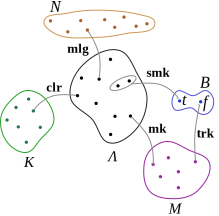
\includegraphics[scale=1.0]{diagramCars}
  \caption{The set $M$ contains all possible makes of cars: Ford,
    Toyota, etc.}
  \label{fig:diagramCars}
\end{figure}

The diagram in the Figure \ref{fig:diagramCars} shows the set $M$ -- the set
of all possible makes of cars. A mapping $\btc{trk}$ returns $true$ if a
given car maker produces trucks.

\subsubsection*{Exercise \ref{exe:relationsGeneral}}
\begin{figure}[htbp]
  \centering
  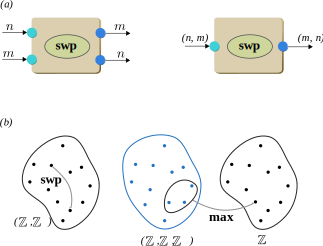
\includegraphics[scale=1.0]{diagramProductSet}
  \caption{(a) Two inputs (outputs) of a function can be replaced with
    a single input of a \bem{pair} of numbers, turning a binary
    function into a unary one. (b) That.}
  \label{fig:diagramProductSet}
\end{figure}

Any binary function can be viewed as a unary function
if two inputs are replaced by a single input of a \emph{pair of
numbers}. Similarly for a function with two outputs. This idea is
illustrated in the Figure \ref{fig:diagramProductSet}(a): The function
{\bf swp} is viewed as a unary function which swaps the numbers in an
\emph{ordered pair}:
\[
\textbf{ swp }\,(n,m) = (m, n)\,.
\]

Given the set $\mathbb{Z}$ of whole numbers, we can create the set of
all possible \emph{ordered pairs} $(n,m)$. This set can be denoted as
follows:
\[
(\mathbb{Z}, \mathbb{Z})\,\textrm{ or }\, \mathbb{Z}\times\mathbb{Z}\,.
\]

The latter notation is standard in mathematics, but the former way
of writing is also acceptable. We can similarly denote the set of all
\emph{ordered triples}:
\[
(\mathbb{Z}, \mathbb{Z}, \mathbb{Z})\,\textrm{ or }\, \mathbb{Z}\times\mathbb{Z}\times\mathbb{Z}\,.
\]

With the notation introduced above, the action of functions with
multiple inputs or outputs can be depicted on the level of sets. The
 Figure \ref{fig:diagramProductSet}(b) shows how this works for the
 functions $\textbf{ swp }$ and $\textbf{ max }$.

